\section{Modèle de Prédiction}\label{Modèle de Prédiction}
Pour prédire le paludisme à partir du jeu de données labélisé obtenue étant donné un nouveau patient, nous utilisons la régression logistique comme \emph{prédicteur}. Dans cette section, nous rappelons brièvement les bases de la fonction de régression logistique. Puisque notre problème est un problème de classification binaire, nous commençons par introduire le problème de classification binaire que nous devons résoudre dans l'étude.
\subsection{Classification Binaire}
Supposons deux classes de diagnostic du paludisme: le \emph{paludisme} et le \emph{non-paludisme}. Nous considérons également \textsc{P} et \textsc{C} comme l’ensemble des patients et un modèle de prédiction. Un patient dans \emph{p} in \textsc{P} est défini par un ensemble de paires $(a_1, v_1), (a_2, v_2), \ldots, (a_n, v_n)$  $a_i$ et $v_i$, pour chaque $1\leq i\leq n$, correspond respectivement à une caractéristique donnée du paludisme et à sa valeur numérique associée définie comme suit.
        
\begin{equation}
v_i = \left\{
\begin{array}{rl}
1 &\text{if $a_i$ is observed} \\
0 &\text{otherwise} \\
\end{array}
\right.
\end{equation}
\begin{definition}{(Notre problème de prédiction)}  Nous définissons notre problème de classification binaire pour la prédiction de la présence ou non du paludisme sur un jeu  de données de patients donné, comme une fonction \textsc{C} qui chaque patient p dans \textsc{P} associe une et une seule classe dans {Paludisme, Non-paludisme}.
Mathématiquement on le note \textsc{C}: \textsc{P} $\mapsto$ \{Paludisme, non paludisme\}
\end{definition}
Dans les cas particulier de notre étude prenons \textsc{C} comme étant la régression logistique
\subsection{Régression logistique}
La régression logistique est une méthode statistique pour effectuer des classifications binaires \cite{Ch14}. Elle prend en entrée des variables prédictives qualitatives et/ou ordinales (par exemple, la présence ou non de fièvre chez  un patient donné) et mesure la probabilité de la valeur de sortie (par exemple, la présence ou pas du paludisme)  en utilisant la \emph{fonction sigmoïde} . La figure \ref{courbe de la fonction sigmoide} montre la forme de la courbe de la fonction Sigmoïde
% The curve of the logistic regression
\begin{figure}[ht]
\centering
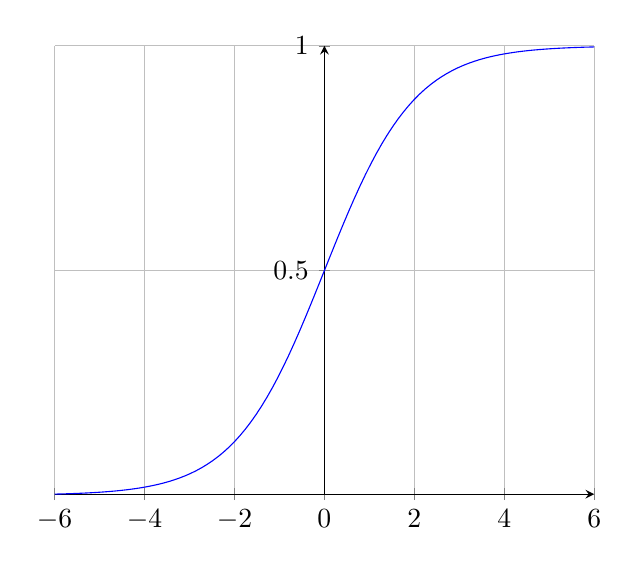
\begin{tikzpicture}
    \begin{axis}%
    [
        grid=major,     
        xmin=-6,
        xmax=6,
        axis x line=bottom,
        ytick={0,.5,1},
        ymax=1,
        axis y line=middle,
    ]
        \addplot%
        [
            blue,%
            mark=none,
            samples=100,
            domain=-6:6,
        ]
        (x,{1/(1+exp(-x))});
    \end{axis}
\end{tikzpicture}
\caption{The curve of the Sigmoid function}\label{sigmoid_curve}
\end{figure}

La régression logistique est un des modèles multivariables couramment utilisé en épidémiologie \cite{Am02,Pr05}  (c’est-à-dire l’étude de l’incidence, de la distribution et du contrôle possible des maladies et d’autres facteurs liés à des problèmes de santé pouvant affecter des groupes de population). Dans un tel contexte la variable dépendante est habituellement la survenue ou non d'un événement (maladie ou autre) et les variables indépendantes sont celles susceptibles d'influencer la survenue de cet événement c'est-à-dire les variables mesurant l'exposition à un facteur de risque ou à un facteur protecteur, ou variable représentant un facteur de confusion. L'intérêt majeur de cette technique est de quantifier la force de l'association entre chaque variable indépendante et la variable dépendante, en tenant compte de l'effet des autres variables intégrées dans le modèle \cite{Am02} .

\subsubsection{Définition fonctionnelle de notre modèle de régression.}
On supposera que la variable  \textsc{Y} à laquelle on s'intéresse est la survenue ou non du paludisme, dont les deux catégories seront notées \textsc{M+} et \textsc{M-}.
Dans le cas particulier d'une seule variable \emph{a} explicative (équivalent d'une régression simple), le modèle s'écrit :
\begin{equation}
\textsc{Pr}(\textsc{M+} ~|~ \emph{a}) = \frac{e^{\alpha + \beta\times \emph{a} }}{1 + e^{\alpha + \beta\times \emph{a} }}
\label{simple_regression}
\end{equation}
où les coefficients $\alpha$ et $\beta$ sont les paramètres du modèle.
\textsc{Pr}(\textsc{M+} ~$|$~ \emph{a})mesure la probabilité d’apparition du paludisme si la variable \emph{a} est observé. La figure \ref{courbe de la fonction sigmoide} représente la fonction logistique correspondante \emph{f(a)}. Encore une fois, l’intérêt principal de cette fonction réside dans la simplicité d’atteindre une estimation des odd ratio (OR) qui mesure la force de l'association entre la maladie \textsc{M} et une variable d'exposition dans une analyse de régression. En effet, si l'exposition est codée en $0$ (la variable n’est pas observée) et$1$ (la variable est observée) comme dans notre cas, le modèle permet d'arriver après simplification à           OR = $e^{\beta}$. Le coefficient $\beta$ de la variable d'exposition dans le modèle logistique est donc le logarithme de l'odds-ratio mesurant l'association entre cette variable (signe ou symptôme) et la maladie (paludisme), ce qui permet d'interpréter facilement les résultats d'une régression logistique.
L'extension vers un modèle à plusieurs variables (régression multiple) se fait très simplement comme le montre la formule ci-dessous
\begin{equation}
\textsc{Pr}(\textsc{M+} ~|~ \emph{$a_1$},\emph{$a_2$}, \ldots, \emph{$a_n$}) = \frac{e^{\alpha + \sum_{i=1}^{n} \beta_i \times \emph{$a_i$} }}{1 + e^{\alpha + \sum_{i=1}^{n} \beta_i \times \emph{$a_i$} }}
\label{multiple_regression}
\end{equation} 
À chaque variable\emph{$a_i$} est associé un coefficient $\beta_i$ et OR$_i$ (mesurant l'association entre Xi et M+) se calcule par  $e^{\beta_i}$.
\subsubsection{Optimisation du modèle.}La question qui se pose généralement lorsqu’on utilise une régression multiple consiste à savoir comment sélectionner l’ensemble minimal de variables parmi les \emph{$a_i$} qui explique mieux la variable \textsc{Y}. Plusieurs stratégies d’optimisation sont possibles pour obtenir le meilleur modèle de prédiction finale qui prend en compte le maximum d'informations tout en restreignant autant que possible le nombre de variables explicatives afin de faciliter l'analyse des résultats. Les plus employées sont les  procédures dites \emph{pas à pas descendantes} ou \emph{pas à pas ascendantes}. Les deux approches appliquent une régression itérative en incluant d’abord dans le modèle la variable qui présente le meilleur coefficient de détermination, puis en ajoutant la variable qui améliore ce coefficient et ainsi de suite pour les méthodes ou pas à pas ascendantes. Pour les méthodes ou pas à pas descendantes, l’ensemble des variables est considéré au début et les variables sont progressivement exclus du modèle, en fonction de ceux qui n’ont pas significativement amélioré le coefficient de détermination.
Dans la section suivante nous présentons les résultats de nos expérimentations obtenues en utilisant notre modèle de régression logistique sur des données réelles de patients









